\chapter{Formal Analysis Using Alloy}
\lstdefinelanguage{Alloy}
{
    morekeywords={fact, abstract,all,and,as,assert,assertion,but,check,disj,else,enum,exactly,expect,extends,for,fun,iden,iff,implies,in,let,lone,module,no,none,not,one,open,or,pred,set,sig,some,sum,univ},
    sensitive=true,
    morecomment=[l]{//},
    morecomment=[s]{/*}{*/},
    morestring=[b]",
    morestring=[b]'
}
\lstset{
    basicstyle=\fontfamily{Roboto}\selectfont\ttfamily\small, % Use Roboto font
    keywordstyle=\color{blue}\textbf,   % Keywords in blue
    commentstyle=\color{gray},   % Comments in gray
    stringstyle=\color{green},   % Strings in green
    showstringspaces=false,
    tabsize=2,
    breaklines=true
}

In this chapter the Alloy model of the CKB system is implemented by describing the main constraints. The aim of the generated world is to underline the constraint about the team size of each battle and the fact that a student can not partecipate to the same battle with two different teams.

\begin{lstlisting}[language=Alloy,  label={lst:alloycode}, basicstyle=\fontfamily{Roboto}\selectfont\ttfamily]
       
    
    open util/relation
    //Signatures
    //DateTime is used to represent a couple <date, time>
    sig DateTime{}
    
    abstract sig Bool {}
    one sig True, False extends Bool {}
    
    /*TestCase represents what the educator will upload when creating a battle in order to test the code of the students*/
    sig TestCase{}
    sig Name{}
    sig Surname{}
    sig Email{}
    sig Password{}
    sig Language{}
    sig Description{}
    sig Rule{}
    sig Title{}
    sig Score{}
    sig RankingTeam{}
    sig RankingStudent{}
    
    /*User is an abstract entity containing all the attributes that each user will have*/ 
    abstract sig User {
        name : disj one Name,
        surname: disj one Surname,
        email: disj one Email,
        password : disj one Password,
    }
    
    //Student represents the STU of the system
    sig Student extends User{
        achievedBadges : set Badge,
        tournaments : set Tournament,
        battles : set Battle
    }
    
    //Educator represents the EDU of the system
    sig Educator extends User{
        ownedTournaments : set Tournament,
        closedTournaments : set Tournament,
        createdBattles : set Battle
    }
    
    /*Tournament entity represents the tournament created by an EDU. In particular, grantedEducators will have all the EDUs who have the same permissions of the creator EDU. "ranking" attribute will contain a map in which the keys will be the STUs and to each key will be assigned a value which is the sum of scores in the battles concerning that tournament */
    sig Tournament {
        id : disj one Int,
        subscriptionDeadline : one DateTime,
        ranking : set RankingStudent, 
        grantedEducators: some Educator,
        battles: disj set Battle,
        studentsSubscribed : set Student,
        badges : set Badge,
    }{
        #studentsSubscribed = #ranking
    }    
    
    /*Battle entity represents the battle created by EDUs in tournaments.
    In particular, the ranking attribute will contain a map in which the keys will be the teams and to each key will be assigned a value which is the score of that team in this battle.
    We use the subscribedTeams attribute instead of subscribedStudents because each team is composed by at least one person and all the components of the team will be subscribed to the battle. 
    As a consequence, we can derive all subscribed STUs by looking at the STUs who appear in the subscribedTeams attribute. */
    sig Battle {
        id : disj one Int,
        creator : one Educator,
        closed : one Bool,
        rankingTeams : disj set RankingTeam,
        manualEvaluation: one Bool,
        language: one Language,
        description:disj one Description,
        testCases: disj some TestCase,
        minStudents : one Int,
        maxStudents : one Int,
        registrationDeadline : one DateTime,
        finalSubmissionDeadline : one DateTime,
        subscribedTeams:disj set Team,
        tournament : one Tournament,
    }{
        #rankingTeams = #subscribedTeams
        
        /*maxStudents and minStudents can't have negative values by definition. */
        maxStudents>0
        minStudents>0 
        
        /*minStudents as a minimum value will be less than or equal to maxStudents by definition */
        minStudents <= maxStudents
        
        /*the registrationDeadline must be earlier than the finalSubmissionDeadline by definition, otherwise it would not be possible to upload code after the registrationDeadline in some cases. */
        registrationDeadline != finalSubmissionDeadline 
    }
    
    /*Team represents the team ( composed by at least one student by definition) created by a student when he subscribes to a battle*/
    sig Team{
        battle : one Battle,
        students: some Student,
    }
    
    /*The entity Badge represents the badges which can be created by EDUs at any moment and can be associated to different tournaments at tournament creation time. */
    sig Badge {
        rules : disj some Rule,
        values : disj some Int,
        title : disj one Title,
    }
    
    //Bool
    pred isTrue[b: Bool] { b in True }
    
    pred isFalse[b: Bool] { b in False }
        
    // Facts
    
    //Battle
    //Subscription to a Battle by a Team
    /*All students subscribed to a battle must be subscribed to the corresponding torunament too. */
    fact subscribedTeamsAreSubscribedToTournament{
        all t: Tournament | all b: Battle | all te : Team | no s: Student | b in t.battles and te in b.subscribedTeams and s in te.students and s not in t.studentsSubscribed
    }
    
    fact teamIsSubscribed{
        all t: Team| all b : Battle | t in b.subscribedTeams <=> b in t.battle
    }
    /*All team subscribed to a battle must satisfy team size constraint of that battle, if the battle is started. */
    fact teamSizeInBoundaries{
        all b: Battle| all t : Team | t in b.subscribedTeams => (#t.students >= b.minStudents and #t.students <= b.maxStudents)
    }    
    
    /*A STU can not participate to the same battle with two different teams.*/
    fact noStudentInTwoTeams{
        all b: Battle, t1 : Team, t2 : Team | no s: Student | t1 in b.subscribedTeams and t2 in b.subscribedTeams and (s in t1.students and s in t2.students) and t1 != t2
    }
        
    /*An Educator has the same privileges of the owner of a tournament if and only if it is a granted EDU for that tournament*/
    fact ownerIsGranted{
        all t: Tournament, e : Educator | t in e.ownedTournaments <=> e in t.grantedEducators
    }
    
    /*A tournament is closed if and only if all its battles are ended*/
    fact closedTournamentclosedBattles{
        all t :Tournament | all b : Battle | t in Educator.closedTournaments <=> (b in t.battles and b.closed = True)
    }
    
    /*A STU is participating to a battle if and only if it is in a subscribed team of that battle*/
    fact inBattleIfInTeam{
        all s : Student | all t: Team | t.battle in s.battles
    }
    
    fact battleCreator{
        all b : Battle | all e : Educator | b.creator = e <=> b in e.createdBattles
    }
    
    fact battlesCreatedInOwnedTournaments{
        all b : Battle | all e : Educator | b in e.createdBattles <=> b.tournament in e.ownedTournaments 
    }
    
    pred show{
        #Battle = 2
        #Badge = 1
        one b : Battle | b.minStudents = 1 and b.maxStudents = 1 and #b.subscribedTeams >1
        one t1 : Team | #t1.students >1
    }
    run show
    
\end{lstlisting}
\section[World]{World}
\begin{figure}[H]
    \centering
    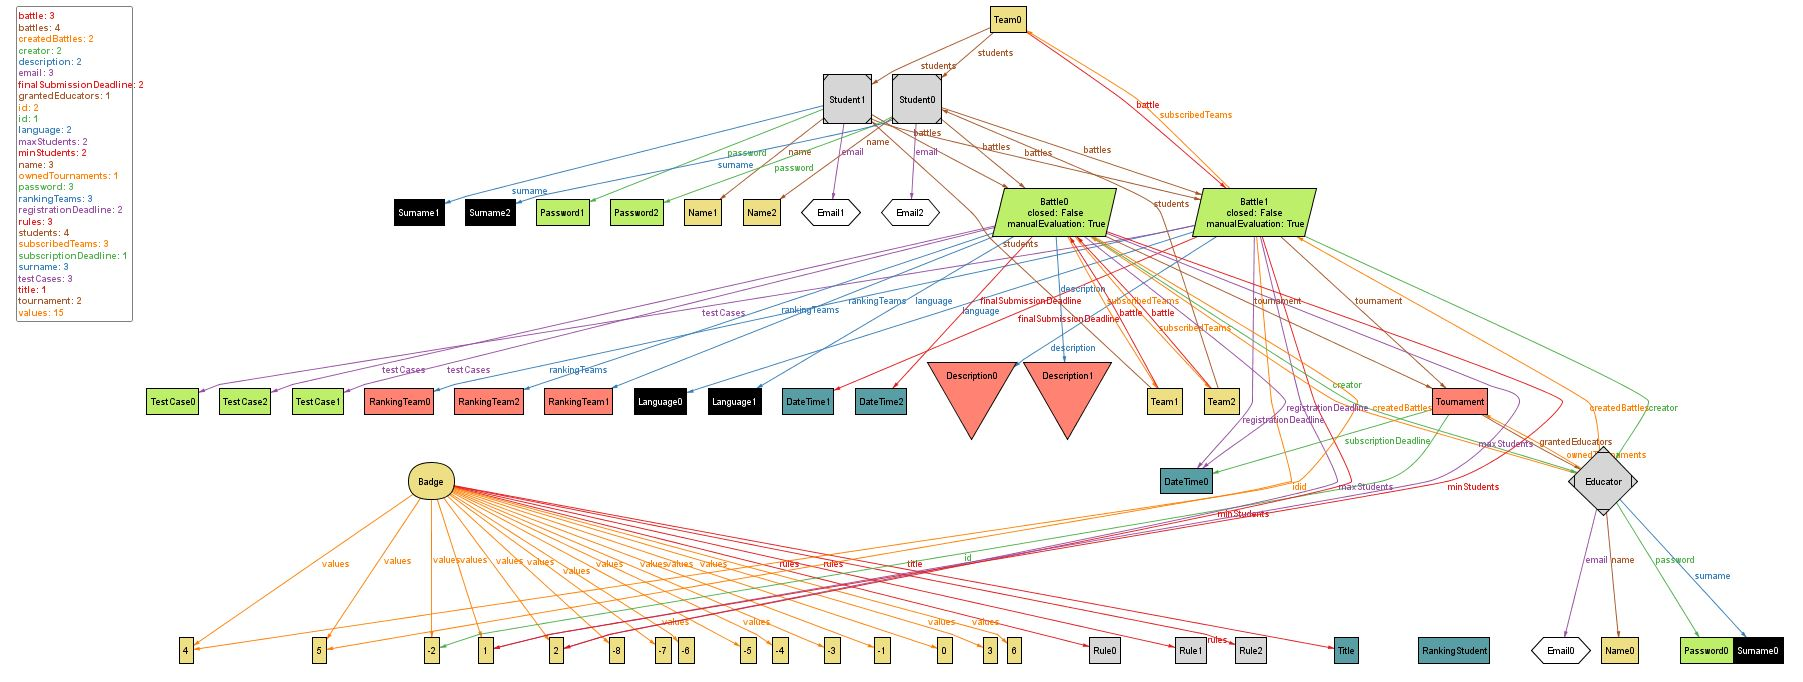
\includegraphics[angle=90,scale = 0.5]{images/alloy/alloy.JPG}
    \caption{World}
\end{figure}